\documentclass{article}
\usepackage{iclr2027_conference}

% ---------------------------------------------------------------------------
% Fonts.  The template calls \usepackage{times}.  Under pdfTeX that resolves
% correctly to Nimbus Roman, but this paper is built with Tectonic (XeTeX),
% where the legacy `times' package does NOT resolve: the body silently falls
% back to Latin Modern and every \textbf/\emph/\textit/\textsc renders as
% upright regular text -- table headers, theorem heads, and section titles
% included.  newtxtext/newtxmath are the maintained Times-compatible
% replacements and resolve correctly under both engines; the embedded body
% face is TeX Gyre Termes, i.e. Times, as the template requires.  If you build
% with pdflatex on a full TeX Live instead, `\usepackage{times}' is equally
% valid -- verify bold and italic in the output either way.
% \openbox and \Bbbk are released because newtxmath and amssymb/amsthm both
% declare them.
% ---------------------------------------------------------------------------
\usepackage{amsmath,amssymb,mathtools}
\usepackage{newtxtext}
\let\openbox\relax
\let\Bbbk\relax
\usepackage[varg]{newtxmath}
\let\openbox\relax
\usepackage{amsthm}
\input{math_commands.tex}

\usepackage{microtype}
\usepackage[hidelinks]{hyperref}
\usepackage{url}
\usepackage{booktabs}
\usepackage{graphicx}
\usepackage{enumitem}
\usepackage{multirow}
\usepackage{tabularx}
\usepackage{array}
\usepackage{xcolor}
\usepackage{algorithm}
\usepackage{algpseudocode}
\usepackage{tikz}
\usetikzlibrary{arrows.meta,positioning,fit,backgrounds,shapes.geometric,calc}
\usepackage{cleveref}
\usepackage{xspace}

% ------------------------------------------------------------------- palette
\definecolor{gacblue}{HTML}{2F6B8A}
\definecolor{gacteal}{HTML}{2A9D8F}
\definecolor{gacred}{HTML}{B4462F}
\definecolor{gacline}{HTML}{3D3D3D}
\definecolor{gacgrey}{HTML}{F4F3F0}

% -------------------------------------------------------------------- macros
\newcommand{\method}{\textsc{GAC}\xspace}
\newcommand{\grc}{\textsc{GRC}\xspace}
\newcommand{\patg}{\textsc{Patg}\xspace}
\newcommand{\code}[1]{\texttt{#1}}
\providecommand{\Description}[1]{}
\newcommand{\retire}{\textcolor{gacred}{\textsc{retire}}\xspace}
\newcommand{\fallback}{\textsc{fallback}\xspace}

% The official math_commands.tex redefines \eqref to "equation~N", which makes
% "Eq.~\eqref{...}" read "Eq. equation 5".  Restore the amsmath form.
\renewcommand{\eqref}[1]{(\ref{#1})}

\theoremstyle{plain}
\newtheorem{proposition}{Proposition}
\theoremstyle{definition}
\newtheorem{definition}{Definition}

% algorithmicx restarts its line counter in every float, which makes hyperref
% emit duplicate ALG@line destinations.  Qualify the anchor with the algorithm
% number so the PDF backend sees unique names.
\makeatletter
\providecommand{\theHALG@line}{\thealgorithm.\arabic{ALG@line}}
\renewcommand{\theHALG@line}{\thealgorithm.\arabic{ALG@line}}
\makeatother
\algrenewcommand\algorithmicrequire{\textbf{Input:}}
\algrenewcommand\algorithmicensure{\textbf{Output:}}
\algrenewcommand{\alglinenumber}[1]{\scriptsize#1:}

\Crefname{algorithm}{Algorithm}{Algorithms}
\crefname{algorithm}{Alg.}{Algs.}

% Let floats fill more of a page.  With five algorithm/figure floats the LaTeX
% defaults strand a third of several pages, which the 9-page limit cannot spare.
\renewcommand{\topfraction}{0.92}
\renewcommand{\bottomfraction}{0.75}
\renewcommand{\textfraction}{0.08}
\renewcommand{\floatpagefraction}{0.80}
\setcounter{topnumber}{3}
\setcounter{totalnumber}{4}
% Caption and float separations are left at the class defaults so the template's
% "one line space before the caption, one line space after the float" rule holds.

\title{From Traces to Guarded Programs: Evidence-Gated Compilation of Recurrent Agent Workflows}

% ===========================================================================
%  AUTHORSHIP AND ANONYMITY  --  READ BEFORE UPLOADING
%
%  ICLR 2027 initial submissions are DOUBLE BLIND.  The switch is the single
%  \iclrfinalcopy line below:
%
%    \iclrfinalcopy present  -> NAMED build.  The author block below is shown.
%                               Use for preprints, arXiv, and circulation.
%    \iclrfinalcopy removed  -> BLIND build.  The style file prints "Anonymous
%                               authors / Paper under double-blind review",
%                               ignores \author entirely, and clears the PDF
%                               author metadata.  Use for the OpenReview
%                               upload.
%
%  As shipped this is the BLIND submission build.  Uncomment \iclrfinalcopy
%  only when preparing a named preprint or camera-ready version.
% ===========================================================================
\author{Reza Rahimi \\
JazzX AI \\
Los Altos, CA, USA \\
\texttt{reza.rahimi@jazzx.ai}}

% \iclrfinalcopy

% Author name reaches the PDF metadata only in the named build, so a blind
% build cannot leak it through `pdfinfo'.
\ificlrfinal
  \hypersetup{pdfauthor={Reza Rahimi}}
\else
  \hypersetup{pdfauthor={}}
\fi
\hypersetup{pdftitle={From Traces to Guarded Programs: Evidence-Gated Compilation of Recurrent Agent Workflows}}

\begin{document}

\maketitle

% \iclrfinalcopy also sets the running head to "Published as a conference paper
% at ICLR 2027".  That is a false claim on an unpublished manuscript, so the
% named build states what this actually is.  The blind build keeps the style
% file's "Under review as a conference paper at ICLR 2027" untouched.
\ificlrfinal\lhead{Preprint. Under review.}\fi

\begin{abstract}
Tool-using agents often invoke a model at every step, even along a repeated read-only
path. Replacing repeated reasoning with deterministic execution could reduce inference
cost, but repetition alone does not make this safe: tool arguments may depend on decisions
not recoverable from observable state, apparently read-only operations may have hidden
effects, and reproducing the same tool calls may still change the agent's final answer.
Recurrence identifies an opportunity for optimization, not permission to remove reasoning.

We introduce \emph{guarded agentic compaction} (\method), a compile-or-retire approach
that converts recurrent execution paths into deterministic programs only when the evidence
supports it. \method grounds every tool argument in the task input or a prior tool result,
treats writes, approvals, handoffs, and unknown effects as hard barriers, protects
compiled execution with input, output, and environment guards, and requires a
finite-sample risk test before deployment. Admission depends jointly on a configured risk
bound and the statistical confidence supported by the available traces. If any requirement
fails, \method keeps the largest justified prefix when possible, or falls back to the
unchanged agent.

Across three live GitHub workflow families and 90 unseen test cases, \method satisfies the
exact task requirements on all 90 cases, compared with 89 of 90 for the unchanged agent,
while reducing model requests by 66.6\%, tokens by 63.1\%, latency by 64.2\%, and estimated
cost by 58.7\%. A time-forward evaluation across five more repositories shows \method
specializing four and refusing the fifth. Experiments on four public trace benchmarks
further show that recurrence and successful replay are not sufficient for specialization.
Under \method's default 0.05 risk bound and associated confidence requirement, NESTFUL,
API-Bank, and BFCL do not provide sufficient qualifying recurrent evidence to establish
that substitution risk is within the admissible bound, so \method conservatively declines
specialization; relaxing the risk or confidence requirements can admit additional
opportunities, making the trade-off between optimization coverage and substitution
assurance explicit. The fourth benchmark demonstrates a distinct limitation: even when
trace evidence supports compilation, the resulting deterministic program can remain
incompatible with the target agent architecture.

\method reframes optimization as evidence-gated specialization: compile only what is
justified, and preserve the agent everywhere else.

\end{abstract}

\section{Introduction}

The standard agent loop pays for a model decision at every tool boundary:
model, tool, model, tool, and so on~\citep{yao2023react}. That flexibility is
valuable while a workflow is novel. At scale, however, mature agents often
revisit the same read-only evidence path with the same data dependencies. In
those settings, repeating the model decision adds latency, tokens, and cost
without necessarily adding useful adaptation.

Removing that decision is not ordinary caching. A tool argument may depend on a
specific earlier observation, a repeated sequence may cross an approval or
write, an apparently read-only tool may hide an undeclared effect, and a
program that replays the same tool outputs may still change the downstream
answer. The problem is therefore not just ``find recurring traces.'' The
problem is to decide when a recurrent model-mediated region can be replaced by a
deterministic program and when it should be refused.

Consider the smallest version of this decision in the benchmark.  A NESTFUL record asks
for the percentage increase from 50 dollars to 60 dollars and records
\code{subtract(60,50) -> divide(result,50) -> multiply(result,100)}.  The trace is
executable and every later argument is grounded in an earlier value, so a recurrence-only
optimizer would have a plausible macro.  The benchmark even supplies successful replay:
across 32 attempted families, 24 held-out windows pass, 12 abstain, and none are wrong.
But after provenance and group filtering the strongest candidate family has only 26
independent groups, while the configured exact gate needs 92 zero-violation groups
($\alpha=.05$, $\delta=.10$, eleven thresholds).  GAC therefore retires every family and
keeps the unchanged agent.  The example makes the distinction concrete: recurrence says
what may be compilable; evidence determines whether replacement is justified.

\begin{figure}[t]
  \centering
  
\includegraphics[width=\linewidth]{../generated_figures/gac_aha_example.pdf}
  \Description{A benchmark-grounded arithmetic trace looks safe to compile, but a
  recurrence-and-replay rule would ship while GAC retires because 26 independent groups
  fall short of the 92-group exact-gate requirement.}
  \caption{The recurrence-versus-admission distinction on NESTFUL.  This is provider-free
  structural compiler evidence, not a live planning or production-safety result.}
  \label{fig:aha-example}
\end{figure}

The benchmark also shows why tool replay is not full substitution evidence.  In an
earlier 18-record GitHub study, a more aggressive three-read artifact had 45/45 clean
tool replays but only 17/18 exact downstream answers: one Markdown URL was lost from the
continuation.  A checked continuation renderer recovered 18/18 in provider-free replay,
but the paper treats that as a detection mechanism rather than a live safety claim.

Framed this way, the closest precedent is not prompt optimization but the
tracing just-in-time compiler. Dynamo~\citep{bala2000dynamo}, trace-based type
specialization~\citep{gal2009tracejit}, and meta-tracing~\citep{bolz2009pypy}
all detect a hot path, compile it behind a \emph{guard}, and deoptimize to the
interpreter when the guard fails~\citep{holzle1992deopt}. Agent traces admit
the same structure --- hot-trace detection becomes family mining, guard
synthesis becomes an entry contract, and deoptimization becomes fallback to the
unchanged agent --- but they add three obligations a JIT does not face. Tool
arguments must be shown to be \emph{grounded} in observable state rather than
invented by the model; declared \emph{effects} must permit speculation, because
an agent's ``interpreter'' can call the outside world; and the residual error
rate of a compiled region is statistical, so it needs a finite-sample bound
rather than a soundness proof.

We study these obligations through \emph{guarded agentic compaction} (\method),
a compile-or-retire trace-to-program system for recurrent read-only prefixes.
The method normalizes executions into a typed episode representation,
reconstructs value provenance for tool arguments, mines recurrent prefix
families, synthesizes bounded programs, induces runtime guards and verifiers,
and admits an artifact only when a finite-sample selective-risk calculation
supports it. Otherwise the baseline agent is retained unchanged
(\cref{fig:pipeline}). The core contribution is thus not ``agent compilation''
in general, but an admissibility argument for trace-derived specialization.

The evidence is deliberately multi-sided. On three distinct GitHub workflow
families with live provider calls, compiled programs preserve or improve exact
held-out task outcomes while reducing requests, tokens, latency, and cost; a
narrower time-forward task then tests transfer across repositories and retains
both success and compile-time retirement. NESTFUL and API-Bank show the
opposite regime, in which recurrent executable traces still fail to justify
deployment. We also retain the strongest practical counterpoint: when a
workflow is already known, hand-written programs can be competitive or tied, so
any claim of automatic superiority would be incorrect.

The paper makes three contributions:
\begin{enumerate}[leftmargin=1.2em,itemsep=1pt,topsep=2pt]
  \item A guarded specialization pipeline (\cref{alg:compile}) that combines
  typed provenance, effect and position barriers, bounded synthesis, runtime
  verification, and finite-sample compile-or-retire admission
  (\cref{alg:calibrate}, \cref{prop:admission}).
  \item A real-provider evaluation across three public-record workflow families,
  plus a narrower cross-repository, time-forward extension that keeps both
  successful artifacts and principled retirements.
  \item A negative-result boundary showing that recurrence and replayability do
  not themselves license deployment: NESTFUL and API-Bank retire under the same
  admission logic, and manual programs constrain any runtime-dominance claim.
\end{enumerate}

\section{Problem Formulation}
\label{sec:problem}

\paragraph{Episodes and candidate regions.}
An episode $E=(z,M,e_{1:T},y)$ contains an entry-state snapshot $z$, a
content-addressed execution manifest $M$, ordered events $e_t$ (model requests
and responses, tool calls and results, handoffs, guardrails, approvals, errors,
commit boundaries), and an observable outcome $y$. Each tool $f$ carries an
application-owned effect declaration $\epsilon(f)$ and capability flags such as
\emph{speculatable}; an unknown effect is not a read.

A candidate region $R=[a,b]$ begins at a model-request boundary and ends after
a tool result. It is \emph{groundable} when every call argument is either an
application-declared literal for that slot or an expression over entry state
or prior results inside $R$,
\begin{equation}
  \forall c_j \in R,\ \forall u \in \operatorname{args}(c_j):\quad
  \operatorname{Lit}(c_j,u)\ \vee\
  \left[u = g_{j,u}\!\left(z, o_{<j}\right),
  g_{j,u}\in\mathcal{L}\right],
  \label{eq:grounding}
\end{equation}
where $\operatorname{Lit}$ is a schema-level allowlist fixed independently of
the traces and $\mathcal{L}$ is a closed, bounded transform library; and
\emph{effect-admissible} when every tool in $R$ is declared read-only,
speculatable, replayable, and inside one principal and isolation partition.
Handoffs, approvals, writes, errors, and unknown effects are hard barriers, not
costs to be traded away. Because the deployed runtime resolves artifacts at the
initial model boundary, the compiler also imposes a \emph{position invariant}:
\begin{equation}
  a = 0 \quad\text{in the normalized model-boundary index.}
  \label{eq:prefix}
\end{equation}
This is not aesthetic. A suffix program dispatched at entry can reorder or
duplicate calls the agent has already made --- a semantic mismatch between
compilation-time and resolution-time position rather than a tuning failure, and
a pilot that violated \cref{eq:prefix} produced exactly that fault
(\cref{app:pilot}).

\paragraph{Selective optimization objective.}
The compiler emits an artifact $A=(P,H,V,q,\eta,M)$: a deterministic program
$P$, hard guard $H$, output verifier $V$, nonconformity score $q$, threshold
$\eta$, and manifest pins $M$. Let $x=(z,M',\omega)$ denote a future entry state,
runtime manifest, and external state. Here $M'\simeq M$ means equality on every
pinned compatibility field; $\omega$ can affect outcomes and cost but is not
observable at the dispatch boundary. Dispatch is \emph{selective},
\begin{equation}
  d_A(x) = \mathbf{1}\{\,H(z,M')=1 \ \wedge\ q(z)\le\eta
              \ \wedge\ M'\simeq M\,\},
  \label{eq:dispatch}
\end{equation}
and any failed precondition runs the unchanged baseline agent $B$. If execution
fails before a commit and staging proves the attempt clean, $B$ runs; a dirty
failure after a commit is an incident, not a fallback. Fix $L(A,x)=1$ for an
externally visible task/contract violation or incident after dispatch; a clean
abort followed by unchanged $B$ has $L=0$. Let $C(A,x)$ include the complete
realized cost of that attempt, including a clean fallback. For a
future group $G=(x_1,\ldots,x_m)$, define
$D_A(G)=\max_i d_A(x_i)$ and
$W_A(G)=\max_i d_A(x_i)L(A,x_i)$. We seek
\begin{equation}
  \max_A\ \ \mathbb{E}\big[d_A(X)\,\{C(B,X)-C(A,X)\}\big]
  \quad\text{s.t.}\quad
  \Pr\!\left[W_A(G)=1 \mid D_A(G)=1\right] \le \alpha .
  \label{eq:objective}
\end{equation}
Two properties shape everything that follows. The constraint conditions on
dispatch: abstention does not enter its denominator, although it earns no
savings in the objective; by convention its conditional risk is zero when
population dispatch probability is zero. Returning \emph{no} artifact is feasible, so
\retire{} is a legitimate output. \Cref{eq:objective} is a design target: the
implementation calibrates a bounded ranked set and retains nondominated
survivors, and we prove neither optimality nor a compiler-wide guarantee for
that search. Calibration uses independent scenario groups as its statistical
units. The group and episode risks coincide in the reported live studies,
where every group contains exactly one public record; they need not coincide
for unequal multi-episode groups.

\section{Guarded Agentic Compaction}
\label{sec:method}

\begin{figure}[t]
  \centering
  % ---------------------------------------------------------------------------
% System architecture of guarded agentic compaction (ICLR single-column build).
%
% Explicit millimetre geometry with anchor=north west so the three lanes cannot
% collide at any scale.  Natural width is ~136mm, which fits the ICLR 5.5in
% (139.7mm) measure without \resizebox, so label sizes stay uniform.
% Colours (gacblue/gacteal/gacred/gacline/gacgrey) are declared in main.tex.
% ---------------------------------------------------------------------------
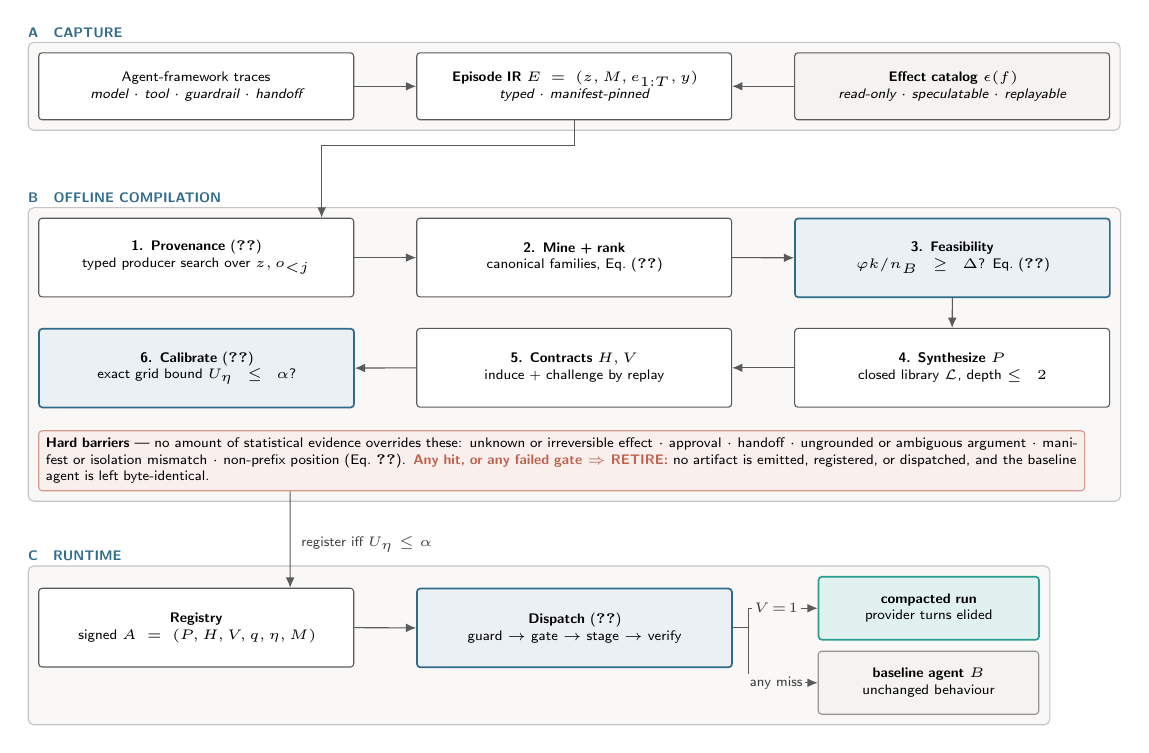
\begin{tikzpicture}[
  x=1mm, y=1mm,
  font=\sffamily\tiny,
  box/.style={
    draw=gacline!85, line width=0.4pt, rounded corners=1.2pt, fill=white,
    anchor=north west, align=center, inner sep=1.6pt,
    minimum width=40mm, minimum height=10mm, text width=36.5mm},
  gate/.style={box, fill=gacblue!10, draw=gacblue, line width=0.6pt},
  good/.style={box, fill=gacteal!14, draw=gacteal, line width=0.6pt,
               minimum width=28mm, text width=25mm, minimum height=8mm},
  base/.style={box, fill=gacgrey, draw=gacline!55,
               minimum width=28mm, text width=25mm, minimum height=8mm},
  frame/.style={draw=gacline!30, line width=0.4pt, rounded corners=2pt,
                fill=gacgrey!55, inner sep=3.6pt},
  barrier/.style={
    draw=gacred!55, line width=0.4pt, rounded corners=1.2pt, fill=gacred!8,
    anchor=north west, align=left, inner sep=2.6pt, font=\sffamily\tiny},
  head/.style={font=\sffamily\bfseries\tiny, text=gacblue,
               anchor=south west, inner sep=0pt},
  flow/.style={-{Latex[length=1.3mm,width=1.1mm]}, draw=gacline!85,
               line width=0.4pt},
  lbl/.style={font=\sffamily\tiny, inner sep=1pt, fill=gacgrey!55,
              text=gacline},
]

% ======================================================= A -- capture (lane 1)
\node[box, minimum height=8.5mm] (sdk) at (0, 0)
  {Agent-framework traces\\\itshape model $\cdot$ tool $\cdot$ guardrail $\cdot$ handoff};
\node[box, minimum height=8.5mm] (ir)  at (48, 0)
  {\textbf{Episode IR} $E=(z,M,e_{1:T},y)$\\\itshape typed $\cdot$ manifest-pinned};
\node[box, minimum height=8.5mm, fill=gacgrey] (cat) at (96, 0)
  {\textbf{Effect catalog} $\epsilon(f)$\\\itshape read-only $\cdot$ speculatable $\cdot$ replayable};

\draw[flow] (sdk.east) -- (ir.west);
\draw[flow] (cat.west) -- (ir.east);

\begin{scope}[on background layer]
  \node[frame, fit=(sdk)(ir)(cat)] (fA) {};
\end{scope}
\node[head] at ([yshift=0.5mm]fA.north west) {A\quad CAPTURE};

% ============================================ B -- offline compilation (lane 2)
\node[box] (prov) at (0, -21)
  {\textbf{1. Provenance} (\cref{alg:patg})\\typed producer search over $z,o_{<j}$};
\node[box] (mine) at (48, -21)
  {\textbf{2. Mine + rank}\\canonical families, Eq.~\eqref{eq:score}};
\node[gate] (feas) at (96, -21)
  {\textbf{3. Feasibility}\\$\varphi k/n_B \ge \Delta$? Eq.~\eqref{eq:ceiling}};

% Row 2 runs right-to-left (serpentine): the stage-3 -> stage-4 hand-off is then a
% short vertical arrow instead of a full-width return line across the barrier band.
\node[box] (synth) at (96, -35)
  {\textbf{4. Synthesize} $P$\\closed library $\mathcal{L}$, depth $\le 2$};
\node[box] (cont) at (48, -35)
  {\textbf{5. Contracts} $H,V$\\induce + challenge by replay};
\node[gate] (cal) at (0, -35)
  {\textbf{6. Calibrate} (\cref{alg:calibrate})\\exact grid bound $U_\eta \le \alpha$?};

\draw[flow] (prov.east) -- (mine.west);
\draw[flow] (mine.east) -- (feas.west);
\draw[flow] (feas.south) -- (synth.north);
\draw[flow] (synth.west) -- (cont.east);
\draw[flow] (cont.west)  -- (cal.east);

\node[barrier, text width=131mm] (bar) at (0,-48)
  {\textbf{Hard barriers} --- no amount of statistical evidence overrides these:
   unknown or irreversible effect $\cdot$ approval $\cdot$ handoff $\cdot$
   ungrounded or ambiguous argument $\cdot$ manifest or isolation mismatch
   $\cdot$ non-prefix position (Eq.~\ref{eq:prefix}).
   \textcolor{gacred!85}{\textbf{Any hit, or any failed gate}
   % Spelled out rather than \retire: Latin Modern Sans has no small-caps face
   % at this size, so \textsc here would trigger a font substitution.
   $\Rightarrow$ \textbf{RETIRE:}} no artifact is emitted, registered, or
   dispatched, and the baseline agent is left byte-identical.};

\begin{scope}[on background layer]
  \node[frame, fit=(prov)(feas)(cal)(bar)] (fB) {};
\end{scope}
\node[head] at ([yshift=0.5mm]fB.north west)
  {B\quad OFFLINE COMPILATION};

% Enters stage B at x=36mm, clear of the lane header and inside the stage-1 box.
\draw[flow] (ir.south) -- ++(0,-3.2) -| (36,-16.4) -- (36,-21);

% ============================================================ C -- runtime lane
\node[box] (reg) at (0, -68)
  {\textbf{Registry}\\signed $A=(P,H,V,q,\eta,M)$};
\node[gate] (disp) at (48, -68)
  {\textbf{Dispatch} (\cref{alg:dispatch})\\guard $\to$ gate $\to$ stage $\to$ verify};
\node[good] (hit) at (99, -66.5)
  {\textbf{compacted run}\\provider turns elided};
\node[base] (miss) at (99, -76)
  {\textbf{baseline agent} $B$\\unchanged behaviour};

\draw[flow] (reg.east) -- (disp.west);
\draw[flow] (disp.east) -- ++(2,0) |- (hit.west)
            node[lbl, pos=0.7] {$V\!=\!1$};
\draw[flow] (disp.east) -- ++(2,0) |- (miss.west)
            node[lbl, pos=0.7] {any miss};

\begin{scope}[on background layer]
  \node[frame, fit=(reg)(disp)(hit)(miss)] (fC) {};
\end{scope}
\node[head] at ([yshift=0.5mm]fC.north west) {C\quad RUNTIME};

% Enters the runtime lane at x=32mm: far enough right that the label clears the
% "C  RUNTIME" lane header, and still inside the Registry box (x = 0..40mm).
\draw[flow] ([xshift=32mm]bar.south west) -- (32,-68)
  node[lbl, pos=0.55, anchor=west, xshift=1mm, fill=none]
  {register iff $U_\eta\le\alpha$};

\end{tikzpicture}

  \caption{Architecture of \method. \textbf{(A)} Capture normalizes traces into
  one typed Episode IR against a declared effect catalog. \textbf{(B)} Offline
  compilation is a cascade of independent rejection points; the shaded band
  lists barriers no statistical evidence can override. \textbf{(C)} At runtime
  exactly one terminal edge compacts; the rest return the unchanged agent.}
  \label{fig:pipeline}
\end{figure}

\begin{algorithm}[t]
\caption{\textsc{Compile} --- the compile-or-retire cascade. Every exit is either a
registered artifact or an attributed \retire, so rejections stay in the denominator.
Stages marked \textsc{(caller)} are separate library entry points run in this order
rather than steps inside one function.}
\label{alg:compile}
\footnotesize
\begin{algorithmic}[1]
\Require episodes $\mathcal{E}$; effect catalog $\mathcal{C}$; entry schema $\Theta$;
         budgets $\alpha,\delta$; grid $\Lambda$; feasibility target $\Delta$
\Ensure artifact $A=(P,H,V,q,\eta,M)$, or \retire{} with an attributed reason
\State $\mathcal{E}\gets\textsc{Qualify}(\mathcal{E},\mathcal{C})$;\quad
       $\{\mathcal{E}_M\}\gets\textsc{PartitionBy}(\mathcal{E},\text{manifest},
       \text{principal},\text{isolation})$
       \Comment{drop partial runs, unpinned manifests}
\ForAll{partitions $\mathcal{E}_M$}
  \State $(\mathcal{T},\mathcal{D},\mathcal{K},\mathcal{S})\gets
         \textsc{GroupedSplit}(\mathcal{E}_M)$ \hfill\textsc{(caller)}
         \Comment{train / dev / calibration / sealed test, split by \emph{group}}
  \State $G\gets\textsc{BuildPatg}(\mathcal{T},\Theta)$ \Comment{\cref{alg:patg}: block
         ungrounded or ambiguous slots}
  \State $\mathcal{F}\gets\textsc{Canonicalize}(\textsc{MineRegions}
         (G,\mathcal{C},w_{\max}))$, keeping only cross-group support
  \If{$\varphi k / n_B < \Delta$} \hfill\textsc{(caller)}
     \State \textbf{record} \retire{} \textbf{(infeasible ceiling, Eq.~\ref{eq:ceiling})};
            \textbf{continue}
     \Comment{try the next compatible partition}
  \EndIf
  \ForAll{families $F\in\mathcal{F}$ ranked by Eq.~\eqref{eq:score}}
    \State $P\gets\textsc{Synthesize}(F,\mathcal{L})$ at depth $\le 2$;\quad
           \textbf{if} $P=\bot$ \textbf{then continue}
           \Comment{ungroundable slot}
    \State $(H,V)\gets\textsc{InduceContract}(F)$;\quad
           \textbf{if} $\neg\textsc{ReplayAndChallenge}(P,V,\mathcal{D})$
           \textbf{then continue} \Comment{counterexample}
    \State $q\gets\textsc{FitScore}(\mathcal{D})$; \textbf{freeze} $q$
           \Comment{dev groups only; never calibration}
    \State $\eta\gets\textsc{Calibrate}(q,H,\mathcal{K},\Lambda,\alpha,\delta)$;\quad
           \textbf{if} $\eta=\bot$ \textbf{then continue}
           \Comment{\cref{alg:calibrate}}
    \State \Return $\textsc{Package}(P,H,V,q,\eta,M)$ with evidence and lifecycle
  \EndFor
\EndFor
\State \Return \retire
\end{algorithmic}
\end{algorithm}


\Cref{fig:pipeline} and \cref{alg:compile} give the same six stages at two
levels of detail. We describe each and state what it can refuse.

\paragraph{1. Typed provenance.}
A capture adapter normalizes framework traces into the Episode IR; manifests
pin prompt, policy, guardrail, tool, model, SDK, tracer, entry-contract, and
effect-catalog identities, and episodes with different compatibility keys are
partitioned before any learning. For each call-argument slot, the
program-argument trace graph (\patg, \cref{alg:patg}) searches entry-state and
prior-result paths for typed values reachable by a bounded transform --- execution
provenance in the database sense~\citep{cheney2009provenance}, specialized to
tool arguments. Two outcomes block a region rather than guessing: a slot with
\emph{no} witness is a genuine model decision, and a slot with more than
$\kappa$ witnesses is ambiguous.

\paragraph{2. Region mining and ranking.}
The miner enumerates model-boundary-to-result windows of at most $w_{\max}$
tool calls, qualifies effects and live-ins, and hashes tool signatures,
dependency topology, run shape, and live-in/live-out shape while abstracting
literal values. Families require support across independent scenario
\emph{groups} rather than raw event frequency, which prevents a single chatty
scenario from manufacturing recurrence. Survivors are ranked by a
minimum-description-length trade-off that pays for expected savings and charges
for heterogeneity, effect exposure, and program size:
\begin{equation}
  \operatorname{score}(F)=
  \underbrace{s_F\,\bar{k}_F\,c_m}_{\text{expected saving}}
  -\lambda_1 H(F)-\lambda_2\rho_{\mathrm{eff}}(F)-\lambda_3|F| ,
  \label{eq:score}
\end{equation}
with $s_F$ the group support, $\bar{k}_F$ the mean removable model requests,
$c_m$ their unit cost, and $H(F)$ the Shannon entropy over canonical variants
inside the family; without $\lambda_1$ the ranking prefers a heterogeneous
family whose single canonical form fits none of its members.
\Cref{eq:score} affects only \emph{which} family is tried first --- no
admission decision depends on it.

\paragraph{3. Feasibility ceiling.}
Before any synthesis runs, an estimator bounds what the compiler could achieve
with a perfect verifier and a gate that never abstains:
\begin{equation}
  \Delta_{\max}=\frac{\varphi\,k}{n_B},
  \qquad\text{necessary:}\quad \varphi\,\rho\,k \ \ge\ \Delta\,n_B ,
  \label{eq:ceiling}
\end{equation}
with $n_B$ baseline model requests per episode, $\varphi$ the fraction of
episodes holding an eligible region, $k$ the requests removed per successful
dispatch, and $\rho$ the verifier pass rate. Since \cref{eq:ceiling} assumes
$\rho=1$, no measured reduction can exceed it, and it is met with equality
exactly when nothing abstains and nothing fails. Reporting it first makes a
decisive negative answer cheap: a workload whose ceiling sits under the target
can be declined without building a compiler for it.

\paragraph{4--5. Bounded synthesis and contracts.}
Synthesis searches a 23-operator library at depth at most two, covering path
selection, indexing, string normalization, arithmetic, comparisons, bounded
collection operations, and narrow loops; bindings are ranked by stability
across groups, and a group-wise refit rejects bindings that exploit row-level
coincidence. The hypothesis space is deliberately small enough to read: the
approach resembles programming-by-example~\citep{gulwani2011flashfill} and
bounded sketching~\citep{solarlezama2006sketching}, and it does \emph{not}
generate arbitrary Python. Hard guards then constrain entry types, required
fields, categorical sets, numeric intervals, patterns, isolation keys, allowed
effects, and manifest pins; verifiers constrain live-out presence, type,
cardinality, empirical hulls, provenance, effect multisets, and call counts.
These are candidate invariants, not proofs for all future inputs --- which is
why a statistical gate follows them rather than replacing them.

\paragraph{6. Exact risk-gated admission.}
\Cref{alg:calibrate} decides deployment. The score $q$ is fitted on \emph{dev}
groups only --- never on calibration groups --- from entry-observable features
such as missing fields, hull margin, temporal drift, and provenance ambiguity,
then frozen together with a finite threshold grid $\Lambda$. For each
$\eta\in\Lambda$ the compiler counts admitted calibration groups ($n_\eta$) and
those containing at least one post-dispatch violation ($k_\eta$), and inverts
the one-sided exact binomial test~\citep{clopper1934binomial} at a
Bonferroni-corrected level, with explicit empty and all-violation cases:
\begin{equation}
  U_\eta=\begin{cases}
  1, & n_\eta=0\ \text{or}\ k_\eta=n_\eta,\\
  \operatorname{Beta}^{-1}\!\left(1-\tfrac{\delta}{|\Lambda|};
  k_\eta+1,n_\eta-k_\eta\right), & 0\le k_\eta<n_\eta,
  \end{cases}
  \quad U_\eta\big|_{k_\eta=0}=1-\left(\tfrac{\delta}{|\Lambda|}\right)^{1/n_\eta}.
  \label{eq:cp}
\end{equation}
It admits the largest-coverage threshold with $U_\eta\le\alpha$ and retires the
family otherwise --- a fixed-grid instance of the learn-then-test
discipline~\citep{angelopoulos2022ltt}. The closed form on the
right is the operative constraint in our experiments: at $\alpha=0.05$, $\delta=0.1$,
and $|\Lambda|=11$, a zero-violation family still needs $n_\eta\ge 92$ admitted
groups. The default output is refusal, not emission.

\begin{algorithm}[t]
\caption{\textsc{Calibrate} --- fixed-grid exact selective admission. The score $q$ and
the grid $\Lambda$ are frozen \emph{before} this procedure sees a calibration group,
which is what makes the union bound legitimate.}
\label{alg:calibrate}
\footnotesize
\begin{algorithmic}[1]
\Require frozen score $q$; hard guard $H$; calibration groups $\mathcal{K}$;
         grid $\Lambda$; budgets $\alpha,\delta$
\Ensure threshold $\eta$ with a simultaneous guarantee, or $\bot$ (\retire)
\State $\mathcal{A}\gets\emptyset$ \Comment{admissible (coverage, threshold) pairs}
\ForAll{$\eta\in\Lambda$}
  \State $K_\eta\gets\{\,g\in\mathcal{K} : \exists z\in g,\ q(z)\le\eta
         \ \wedge\ H(z)=1\,\}$;\quad $n_\eta\gets|K_\eta|$;\quad
         \textbf{if} $n_\eta=0$ \textbf{then continue}
         \Comment{vacuous bound $U_\eta=1$}
  \State $k_\eta\gets|\{\,g\in K_\eta : g\ \text{contains a violation}\,\}|$
         \Comment{\emph{wrong after dispatch} only, never abstention}
  \State $U_\eta\gets\operatorname{Beta}^{-1}\!\big(1-\tfrac{\delta}{|\Lambda|};\,
         k_\eta+1,\ n_\eta-k_\eta\big)$;\quad
         \textbf{if} $U_\eta\le\alpha$ \textbf{then}
         $\mathcal{A}\gets\mathcal{A}\cup\{(n_\eta/|\mathcal{K}|,\eta)\}$
         \Comment{Eq.~\eqref{eq:cp}}
\EndFor
\State \Return $\bot$ if $\mathcal{A}=\emptyset$, else
       $\arg\max_{(\mathrm{cov},\eta)\in\mathcal{A}}\ \mathrm{cov}$
       \Comment{largest coverage among certified thresholds}
\end{algorithmic}
\end{algorithm}


\begin{proposition}[Per-candidate selective-risk admission]
\label{prop:admission}
Fix one candidate program, hard guard, verifier, score, group-level violation
rule, and finite grid $\Lambda$ before calibration. If calibration groups are
i.i.d. from the future-group distribution, then with probability at least
$1-\delta$, every $\eta\in\Lambda$ satisfies $r_\eta\le U_\eta$, where
$r_\eta$ is post-dispatch group risk. Hence the selected threshold satisfies
$r_\eta\le\alpha$ whenever $U_\eta\le\alpha$.
\end{proposition}

\Cref{app:proof} gives the proof. The guarantee is deliberately narrow: it is
\emph{per fixed candidate}, not compiler-wide over the adaptive candidate
search \cref{alg:compile} actually performs, and it conditions on group
exchangeability rather than establishing it (\cref{sec:discussion}). The
scientific point is that guarded deployment requires an explicit evidence
boundary, not just a recurrent trace and a successful replay.

\section{Experimental Setup}
\label{sec:setup}

Because the claim is an \emph{admissibility} claim, the evaluation asks three
questions: does specialization preserve outcomes while saving work on real
records (\cref{sec:res-primary})? Does it transfer under a time-forward split
(\cref{sec:res-multirepo})? And does it refuse when evidence is thin
(\cref{sec:res-refusal})?

\subsection{Benchmark at a glance}
\label{sec:benchmark}

Every GitHub sample begins with one issue or pull-request number from a pinned
public snapshot. The agent must make read-only calls and return exact,
source-grounded fields, not a subjective preference. The three primary families
use 132 discovery and 30 balanced held-out records each, with live provider
calls. \Cref{tab:benchmark-glance} shows what one sample asks an agent to read
and return; it tests both the structured answer and whether its evidence remains
available after compaction.

\begin{table}[t]
  \centering
  \caption{Primary GitHub benchmark at a glance. Each sample supplies one record
  number from a pinned public snapshot; every listed answer field is checked
  against the source record.}
  \label{tab:benchmark-glance}
  \footnotesize
  \setlength{\tabcolsep}{2.5pt}
  \renewcommand{\arraystretch}{1.12}
  \begin{tabularx}{\linewidth}{@{}p{0.16\linewidth}>{\raggedright\arraybackslash}X>{\raggedright\arraybackslash}X@{}}
    \toprule
    Task & Read-only evidence path & Exact answer contract \\
    \midrule
    Issue type & \code{issue\_number} $\rightarrow$ record, official labels,
    comments & Title, state, label-derived category, verbatim excerpt \\
    PR outcome & \code{pr\_number} $\rightarrow$ PR record, merge status,
    discussion & \code{open}, \code{merged}, or \code{closed\_unmerged}, plus
    title and comment excerpt \\
    Backlog attention & \code{issue\_number} $\rightarrow$ open-issue record,
    assignees, discussion & \code{owned}, \code{discussed\_unowned}, or
    \code{awaiting\_first\_response}, plus title, owner, and excerpt \\
    \bottomrule
  \end{tabularx}
\end{table}

\paragraph{Cross-repository time-forward extension.}
A narrower two-read PR-outcome task spans five frozen public repositories.
Held-out records are strictly newer than discovery records, and selection is
sealed before provider calls; repositories without an admitted artifact remain
in the result. A balanced rerun on three repositories controls the
\code{open}/\code{merged}/\code{closed\_unmerged} mix.

\paragraph{External refusal benchmarks.}
NESTFUL and API-Bank supply valid executable traces whose evidence is still
insufficient; they retain the argument-level producer structure that provenance,
synthesis, replay, and admission need, and they measure none of them as live
planning quality~\citep{basu2025nestful,li2023apibank}.

\paragraph{Conditions, metrics, and statistics.}
Each GitHub family compares the unchanged baseline $B$, the compiled artifact,
and a hand-written pre-model program on the same records, so the comparison is
paired rather than across cohorts. Quality is exact task-contract satisfaction;
resources are requests, interfaces, tokens, latency, and estimated cost. We use
paired exact McNemar tests, bootstrap intervals, and Wilcoxon signed-rank tests;
the only guaranteed multiplicity control is the Bonferroni term in
\cref{eq:cp}. All admission runs use $\alpha=0.05$, $\delta=0.1$, and
$|\Lambda|=11$ (\cref{app:config}).

\section{Results}

\subsection{Primary workflows: preserved contracts, less work}
\label{sec:res-primary}

\begin{table}[t]
  \centering
  \caption{Primary live-provider results ($n=30$ held-out records per family).
  ``Interfaces'' counts provider-visible tool interfaces. All conditions see
  identical records, model, and grader; \emph{Manual} is hand-written with full
  knowledge of the workflow.}
  \label{tab:primary}
  \footnotesize
  \setlength{\tabcolsep}{3.5pt}
  \begin{tabular}{@{}lccccccccc@{}}
\toprule
& \multicolumn{3}{c}{Exact held-out contract} & & \multicolumn{5}{c}{Reduction of compiled vs.\ baseline (\%)} \\
\cmidrule(lr){2-4}\cmidrule(lr){6-10}
Family & Base & Compiled & Manual & & Requests & Interfaces & Tokens & Latency & Cost \\
\midrule
Issue-type routing        & 30/30 & \textbf{30/30} & 30/30 & & 50.0 &  0.0 & 39.5 & 51.7 & 32.0 \\
PR-outcome audit          & 30/30 & \textbf{30/30} & 30/30 & & 75.0 & 66.7 & 80.8 & 73.0 & 75.3 \\
Backlog-attention routing & 29/30 & \textbf{30/30} & 30/30 & & 74.8 & 66.3 & 81.4 & 68.9 & 75.1 \\
\midrule
Weighted total ($n=90$)   & 89/90 & \textbf{90/90} & 90/90 & & 66.6 & 44.2 & 63.1 & 64.2 & 58.7 \\
\bottomrule
\end{tabular}

\end{table}

Across the 90 held-out records, \method satisfies 90/90 exact contracts versus
89/90 for the unchanged agent (\cref{tab:primary}), reducing provider requests by
66.6\%, tokens by 63.1\%, latency by 64.2\%, and estimated cost by 58.7\% in
aggregate. Issue-type routing admits only a two-read prefix, whereas the two
deeper workflows approach 75\% fewer requests.

No held-out record is a compiled-only failure; the one-sided 95\% upper bound on
that discordance is 3.3\%, which supports preservation on the observed cohort, not
equivalence in general. Each artifact was admitted with 92 zero-violation
calibration groups ($U_\eta=0.0498\le.05$). Hand-written programs also achieve
90/90 and are cheaper for issue-type routing.

\subsection{Time-forward transfer: compile or retire}
\label{sec:res-multirepo}

On a narrower two-read pull-request outcome task across frozen public
repositories, with held-out records strictly newer than discovery records and
selection sealed before any provider call, \method completes 120/120 exact
held-out pairs on four of five repositories and retires \code{pytorch/pytorch} at
compile time rather than loosening its gate; requests fall 44.4\% and tokens
52.4\%. A balanced three-repository rerun reaches 180/180 exact pairs at 66.7\%
fewer requests and 78.4\% fewer tokens
(\cref{tab:multirepo-disaggregated}). A fixed two-read template is more efficient
in the five-repository core and essentially tied in the rerun, so this is again
evidence of automatic discovery and principled retirement rather than of runtime
dominance.

\subsection{What binds: sample size, then deployability}
\label{sec:res-refusal}

\begin{table}[t]
  \centering
  \caption{Where refusal happens, and what happens where it does not. Stage
  numbers are \cref{alg:compile}'s; ``slots'' is the share of dependency slots with
  a recovered producer, ``p/a/w'' means held-out replay pass/abstain/wrong, and
  $n_{\max}$ is the largest family support against the 92 \cref{eq:cp} requires.}
  \label{tab:funnel}
  \footnotesize
  \setlength{\tabcolsep}{4pt}
  \begin{tabular}{@{}lccc@{}}
\toprule
Stage of \cref{alg:compile} & NESTFUL & API-Bank & BFCL v4 \\
\midrule
Episodes / recorded traces                          & 1{,}415 & 212 & 200 \\
Tools compilable / effect-blocked                   & ---     & 21 / 28 & 34 / 47 \\
\addlinespace[1pt]
Dependency slots with producer recovered (1)        & 5{,}531 / 5{,}746 (96.3\%) & 559 / 881 (63.5\%) & 1{,}445 / 2{,}124 (68.0\%) \\
Episodes yielding an admissible window (2)          & 1{,}207 (85.3\%) & 37 (17.5\%) & 86 (43.0\%) \\
Families at or above the support floor (2)          & 32 & 8 & 9 \\
Families that synthesize a program (4)              & 12 & 2 & 4 \\
Held-out replay: pass / abstain / \textbf{wrong} (5)& 24 / 12 / \textbf{0} & 0 / 2 / \textbf{0} & 3 / 3 / \textbf{0} \\
\addlinespace[1pt]
Largest family support $n_{\max}$ (6)               & 26 & 8 & 15 \\
\textbf{Artifacts admitted}                         & \textbf{0} & \textbf{0} & \textbf{0} \\
\bottomrule
\end{tabular}

\end{table}

The external substrates isolate the binding constraint (\cref{tab:funnel}). All
four clear provenance, synthesis, and held-out replay with \emph{no} wrong
execution anywhere. NESTFUL, API-Bank, and executed BFCL gold plans then retire,
and each retirement was arithmetically settled before the compiler ran---which is
why a fourth substrate was needed. AppWorld's public gold solutions reach
$n_{\max}=136$, so it is the first external corpus where \cref{eq:cp} is
satisfiable, and it admits one artifact at 92/92 zero-violation groups
($U_{\hat\eta}=0.0498$) with 11/11 exact held-out replay, under both
pre-registered effect arms. Two features bound it: the gate is step-like, and the
admitted program is argument-free, so provenance fixed its \emph{length} rather
than its content---four further candidates retired, two on 89 and 90 eligible
groups at $U=0.051$, and one mined three calls but synthesized two because its
login password slot is not groundable in every supporting group
(\cref{app:external}).

Admissibility is not dispatchability. Gold solutions are not agent
trajectories, so we also test the admitted region against AppWorld's 28 released
baseline runs. Over 8{,}190 held-out trajectories it is structurally eligible at
the entry boundary in $37.9\%$, and that average is bimodal: near-total for
full-code agents, and $1$ of $4{,}680$ for ReAct and plan-and-execute, which open
by reading API documentation so the prefix leaves position~0
(\cref{tab:appworld-dispatch}). These trajectories repeat tasks across 28 released
runs and are descriptive units, not 8{,}190 independent samples. A miss abstains
cleanly, and this measurement bounds $\phi$ from above rather than estimating a
population dispatch rate, so no saving or inferential interval is claimed.

\section{Related Work}
\label{sec:related}

\paragraph{Guarded trace and agent workflow compilation.}
\method adapts the tracing-JIT pattern---compile a hot path behind a guard and
return to the interpreter on a miss~\citep{bala2000dynamo,holzle1992deopt}---to
agents, whose arguments must remain grounded in observed state and whose
speculation must be licensed by declared effects~\citep{lucassen1988effects}.
Recent systems mine meta-tools, induce workflows, cache plans, compile typed
orchestration, validate tool-state plans, search workflow graphs, or prune
multi-agent topology
\citep{abuzakuk2026awo,wang2025awm,zhang2025plancache,wei2026evoc2f,winston2026agentjit,li2026flowcompile,chen2026agentslimming}.
They share our premise that recurrence is exploitable and differ in what they
demand before exploiting it. The delta is three-fold. \emph{First}, they take a
recurring subsequence as the unit; we take the subsequence as a proposal and the
argument-level witness as the unit, which is why the motivating region shrinks
from three reads to two instead of being accepted or dropped whole.
\emph{Second}, their guards test the input, whereas ours are a cascade in which
provenance, effects, position, contracts, and a finite-sample bound each hold a
veto --- so a candidate can fail for reasons no additional trace evidence can
repair. \emph{Third}, they report what compilation achieved, whereas a compile-or-retire
system must also report what it refused.

\paragraph{Other optimization targets.}
DSPy optimizes prompts, GEPA evolves them, RouteLLM changes models, and
LLMCompiler parallelizes current calls
\citep{khattab2024dspy,agrawal2026gepa,ong2025routellm,kim2024llmcompiler}.
\method instead replaces a historical boundary only after guarded evidence.

\paragraph{Synthesis, risk control, and evaluation.}
The bounded search draws on programming by example, sketching, and execution
provenance~\citep{gulwani2011flashfill,solarlezama2006sketching,cheney2009provenance};
admission uses a Clopper--Pearson bound with fixed-grid learn-then-test, not a
new bound~\citep{clopper1934binomial,angelopoulos2022ltt}. BFCL and ToolLLM
score tool use broadly~\citep{patil2025bfcl,qin2023toolllm};
NESTFUL and API-Bank retain the producer references and call results needed for
post-trace provenance, replay, and refusal~\citep{basu2025nestful,li2023apibank}.

\section{Discussion and Limitations}
\label{sec:discussion}

The strongest supported claim is narrow but meaningful: repeated read-only
workflow prefixes can be specialized into guarded deterministic programs that
preserve exact held-out contracts on several real GitHub families while failing
closed when evidence is inadequate --- stronger than a token-savings report,
because the same artifact retains principled retirements on NESTFUL, API-Bank,
and one cross-repository cohort.

\paragraph{Gate maturity is the main scientific risk.}
\Cref{prop:admission} is per-candidate, not compiler-wide over the adaptive
family search of \cref{alg:compile}, so the certificate is conditional on
freezing the candidate relative to calibration. The gate is also step-like
empirically: it behaves as an all-or-none support test at $n_\eta\ge 92$ rather
than tracing a risk--coverage frontier, so we have shown that the rule
\emph{refuses} correctly far better than that $q$ \emph{discriminates}.
Refitting $q$ so the registered gate yields a genuine frontier is the
highest-value follow-up.

\paragraph{External validity and practical competitiveness.}
The richer workflow-family evidence comes from one revision-pinned repository
snapshot and one provider/model family, and the cross-repository extension
broadens scope only on a narrower task where a fixed template is essentially
tied; we establish no superiority on full cross-repository workflows, under
drift, or across providers. Hand-written programs also remain competitive when
the workflow is already known, and we do not measure manual authoring or
maintenance cost --- a complete comparison would price the engineering axis
too.

\paragraph{Semantic scope.}
Exact task contracts do not certify semantic equivalence of the final answer
once a model continuation follows; counterfactual trace
auditing~\citep{zhou2026cta} would detect the gap. Writes, handoffs, hosted
tools, and undeclared effects sit outside \cref{prop:admission} entirely, and
removing a model turn can remove a guardrail evaluation that ran at that turn
--- boundaries that are the conditions for an honest guarded deployment story,
not accidents of the implementation.

\section{Conclusion}

\method treats recurrence as candidate evidence, not permission to rewrite an
agent. Across live GitHub families and a cross-repository extension it saves
resources while preserving exact held-out contracts; on three external
benchmarks it refuses. Judge workflow optimizers by their evidence,
refusals, and fallback---not only the turns they remove.


\section*{AI Use Statement}
In preparing this submission, the authors used generative AI tools to help
restructure the manuscript, improve readability, suggest section organization,
draft and revise parts of the paper text, critique methodological exposition
and internal consistency, and convert repository-grounded results into LaTeX
tables and submission materials. We did not use generative AI tools to generate
experimental results or to replace manual verification of claims. All reported
numbers, citations, equations, and comparisons were checked against the
repository artifacts, retained outputs, and source files, and the authors take
responsibility for the final content of the paper.

\section*{Ethics Statement}
This paper studies methods for removing model-mediated decisions from
tool-using agents. The main risk is over-trusting a compiled prefix and thereby
accelerating unsafe automation or silently removing safeguards; deleting a
model boundary can also delete a guardrail evaluation that happened to run at
that boundary. Our method mitigates this risk by compiling only read-only
prefixes, treating unknown effects, approvals, handoffs, and writes as hard
barriers, and defaulting to retirement or fallback when evidence is
insufficient. All study data are public records (GitHub repository metadata)
or public benchmarks; no personal or private data were collected. The reported
artifact is not a license to bypass human review, legal or compliance controls,
or safety guardrails in high-stakes domains; unsupported regimes are part of
the result, not exceptions to hide.

\section*{Reproducibility Statement}
The main paper reports exact cohort sizes, evaluation protocols, quantitative
metrics, and the claim boundaries attached to each study.
\Cref{alg:compile,alg:calibrate} give the deployed compiler and admission rule;
\Cref{alg:patg,alg:dispatch} in the appendix give provenance construction and
runtime dispatch. \Cref{app:proof} proves \Cref{prop:admission}, and
\Cref{app:config} lists every hyperparameter used by the reported runs. The
repository contains source manifests, raw result files, deterministic table and
figure generation, and scripts for the live GitHub studies, the
cross-repository extension, NESTFUL, and API-Bank. For anonymous submission,
the code and retained artifacts should be packaged as an anonymous
supplementary archive with hashes and manifests preserved.

\bibliographystyle{iclr2027_conference}
\bibliography{references}

\clearpage
\appendix
\section{Proof of \texorpdfstring{\Cref{prop:admission}}{Proposition 1}}
\label{app:proof}

Condition on the train/development data, fix $\eta\in\Lambda$, and write
$\gamma=\delta/|\Lambda|$. Let $D_i^\eta$ and $W_i^\eta$ be the group admission
and violation indicators defined in \cref{sec:problem}. Because the entire
candidate and grid were frozen before calibration and groups are i.i.d., the
pairs $(D_i^\eta,W_i^\eta)$ are i.i.d. Conditional on $n_\eta=m>0$ admitted
groups, their violation count therefore satisfies
$k_\eta\mid n_\eta=m\sim\operatorname{Binomial}(m,r_\eta)$, where
$r_\eta=\Pr(W^\eta=1\mid D^\eta=1)$. Inverting the one-sided exact binomial
test~\citep{clopper1934binomial} gives the upper bound
$U_\eta=\operatorname{Beta}^{-1}(1-\gamma;\,k_\eta+1,\,m-k_\eta)$ of
\cref{eq:cp}, which satisfies
$\Pr\{r_\eta > U_\eta \mid n_\eta=m\}\le\gamma$. When $m=0$ the event is
impossible under the convention that empty-admission thresholds receive the
vacuous bound $U_\eta=1$. Averaging over the random value of $n_\eta$ therefore
yields $\Pr\{r_\eta > U_\eta\}\le\gamma$ for each fixed threshold. Applying the
union bound over the finite grid gives
$\Pr\{\exists\eta\in\Lambda: r_\eta > U_\eta\}\le|\Lambda|\gamma=\delta$, i.e.
simultaneous coverage with probability at least $1-\delta$. On that event,
every threshold whose upper bound is at most $\alpha$ satisfies the group-level
target in \cref{eq:objective}, including the threshold returned by
\cref{alg:calibrate}. $\qquad\blacksquare$

Two scope conditions are worth restating. First, the statement is
\emph{per fixed candidate}: \cref{alg:compile} may calibrate several families
and retain survivors, and that outer search is not multiplicity-corrected.
Second, i.i.d.\ source groups is an assumption about
the calibration cohort, not a property the compiler verifies; the grouped split
in \cref{alg:compile} makes it plausible by construction but does not establish
it under temporal drift.

\section{Additional Algorithms}
\label{app:algorithms}

\begin{algorithm}[t]
\caption{\textsc{BuildPatg} --- typed argument provenance. A slot with no witness is a
genuine model decision; a slot with too many witnesses is ambiguous. Both block the
region rather than defaulting to the cheapest explanation.}
\label{alg:patg}
\footnotesize
\begin{algorithmic}[1]
\Require episodes $\mathcal{T}$; entry schema $\Theta$; transform library $\mathcal{L}$;
         ambiguity cap $\kappa$
\Ensure provenance graph $G$ with one edge per grounded argument slot
\State $G\gets\emptyset$
\ForAll{episodes $E=(z,M,e_{1:T},y)\in\mathcal{T}$}
  \State $\Sigma\gets\{(\text{``}z\text{''},\pi,v) : (\pi,v)\in\textsc{Flatten}(z),\,
         \pi\in\Theta\}$ \Comment{only allowlisted entry paths are eligible}
  \ForAll{tool calls $c_j\in e_{1:T}$ in order}
    \ForAll{argument slots $u\in\operatorname{args}(c_j)$}
      \State $\mathcal{H}\gets\{\,\sigma\in\Sigma : \exists\,g\in\mathcal{L},\;
             g(\sigma)=u,\ \operatorname{depth}(g)\le 2\,\}$
      \If{$u$ is declared \emph{literal-only} for $c_j$}
        \State $\mathcal{H}\gets\{\sigma\in\mathcal{H} : g=\mathrm{id}
               \ \text{or}\ g\ \text{constant}\}$
               \Comment{never reconstruct a page index or a limit}
      \EndIf
      \If{$\mathcal{H}=\emptyset$}
        \State \textbf{mark} $c_j$ \textsc{model-originated}; \textbf{block} region
      \ElsIf{$|\mathcal{H}|>\kappa$}
        \State \textbf{mark} $c_j$ \textsc{ambiguous}; \textbf{block} region
      \Else
        \State $G\gets G\cup\{\sigma\xrightarrow{\,g\,}(c_j,u)\}$ for the
               minimum-description-length $\sigma$
      \EndIf
    \EndFor
    \State $\Sigma\gets\Sigma\cup\{(\operatorname{var}(c_j),\pi,v) :
           (\pi,v)\in\textsc{Flatten}(o_j)\}$
           \Comment{a result witnesses only \emph{later} slots}
  \EndFor
  \ForAll{pairs $(e_s,e_t)$ sharing a resource where either writes it}
    \State $G\gets G\cup\{e_s\prec e_t\}$
           \Comment{order edge: no reordering is ever proposed across a conflict}
  \EndFor
\EndFor
\State \Return $G$
\end{algorithmic}
\end{algorithm}

\begin{algorithm}[t]
\caption{\textsc{Dispatch} --- boundary-time admission. Cheap deterministic checks reject
first and the calibrated gate runs only on what survives them. Exactly one exit path
compacts; the rest return the unmodified agent, and only a dirty post-commit failure
raises an incident.}
\label{alg:dispatch}
\footnotesize
\begin{algorithmic}[1]
\Require entry state $z$; runtime context $M'$; registry $\mathcal{R}$;
         mode $m\in\{\textsf{off},\textsf{shadow},\textsf{live}\}$
\Ensure observations for the region, or \fallback{} to the baseline agent $B$
\If{$m=\textsf{off}$} \State \Return \fallback
    \Comment{conformance: model-visible input must be byte-identical}
\EndIf
\State $A\gets\mathcal{R}.\textsc{Resolve}(M'.\text{compatibility},M'.\text{partition})$
\If{$A=\bot \ \vee\ A.\text{lifecycle}\neq\textsc{Active}
     \ \vee\ \neg\textsc{VerifySignature}(A)$}
  \State \Return \fallback
\EndIf
\If{$H_A(z,M')\neq 1$} \State \Return \fallback
    \Comment{manifest pins, isolation keys, typed hulls, effect set}
\EndIf
\If{$\operatorname{tools}(A.P)\cap\textsc{AlreadyObserved}\neq\emptyset$}
  \State \Return \fallback
    \Comment{the region already ran; its live-ins are not the fitted ones}
\EndIf
\If{$m=\textsf{live} \ \wedge\ \exists f\in\operatorname{tools}(A.P):
     \mathcal{C}(f).\textit{quota\_attested} \wedge \textsc{Snapshot}=\bot$}
  \State \Return \fallback
    \Comment{no staging owner, so a discarded attempt is not attestable}
\EndIf
\If{$q_A(z)>\eta_A$} \State \Return \fallback
    \Comment{calibrated abstention on an uncertain input}
\EndIf
\If{$m=\textsf{shadow}$}
  \State \textbf{log} would-dispatch; \Return \fallback
    \Comment{observe coverage without changing behaviour}
\EndIf
\State $S\gets\textsc{Stage}.\textsc{Begin}()$;\quad
       $r\gets\textsc{Interpret}(A.P,z,\textsc{Facade}(\mathcal{C}))$
       \Comment{the facade re-checks effects at execution time}
\If{$r$ raised \textsc{PreCommitError}}
  \State \textbf{assert} $S.\textsc{Reversible}()$; \Return \fallback
\ElsIf{$r$ raised \textsc{PostCommitError}}
  \State \Return \textsc{Incident}
    \Comment{an external commitment happened; do not feign rollback}
\EndIf
\If{$V_A(r)\neq 1$}
  \State \textbf{discard} $r$; \Return \fallback
    \Comment{live-outs, effect multiset, and call count are checked before use}
\EndIf
\State $S.\textsc{Commit}(r.\text{effects})$;\quad \Return $r.\text{observations}$
\end{algorithmic}
\end{algorithm}


\Cref{alg:patg} constructs the typed provenance graph that decides
\cref{eq:grounding}. Its two block conditions are asymmetric on purpose: a slot
with no witness is treated as a genuine model decision and a slot with more
than $\kappa$ witnesses is treated as ambiguous, so the analysis never resolves
an argument by picking the cheapest available explanation.

\Cref{alg:dispatch} is the runtime counterpart of \cref{eq:dispatch}. Cheap
deterministic checks reject first and the calibrated gate runs only on what
survives them, so the common case costs a registry lookup and a guard
evaluation. Exactly one exit path compacts; every clean rejection returns the
unmodified baseline agent, and any failure whose reversibility cannot be
attested raises an incident rather than feigning a rollback. ``Baseline'' is
byte-exact only where a staging owner holds
the commit boundary: the outer runner can restore byte-identical model input,
whereas a model-boundary adapter cannot un-emit a response the host has already
committed to conversation history.

\section{Configuration}
\label{app:config}

All reported admission runs use risk budget $\alpha=0.05$, confidence budget
$\delta=0.1$, and a fixed grid of $|\Lambda|=11$ thresholds, which fixes the
zero-violation sample requirement at
$n_\eta\ge\log(\delta/|\Lambda|)/\log(1-\alpha)=91.6$, i.e.\ 92 admitted
groups; at exactly $n_\eta=92$ and $k_\eta=0$ the bound is
$U_\eta=1-(0.1/11)^{1/92}=0.0498\le\alpha$. Tightening the confidence budget to
$\delta=0.05$ would raise the requirement to 106 groups, which no study in this
paper reaches, so $\delta=0.1$ is the operative setting throughout and is
reported as such rather than rounded to match $\alpha$. A Bonferroni repair over
$m=2$ candidate families would use $\gamma=\delta/(m|\Lambda|)$ and land on the
same 106-group requirement, which is why the paper reports per-candidate
certificates rather than a compiler-wide one. The grid is
$\Lambda=\{.02,.05,.08,.11,.14,.17,.20,.25,.30,.40,.50\}$ and the ambiguity cap
is $\kappa=3$.
Synthesis uses a 23-operator closed library at depth $\le 2$; region mining
uses $w_{\max}$ tool calls per window and requires support across independent
scenario groups. The implementation also supports a minimum-distinct-days
requirement, which the single-snapshot live study does not exercise
(\code{min\_days}\,=\,1). Two terms of \cref{eq:score} are coarser in the
implementation than the notation suggests: $\rho_{\mathrm{eff}}$ is
approximated by the fraction of tool names containing a namespace separator
rather than read from the effect catalog, and $|F|$ is substituted by the
argument-slot count of the first observed window because ranking precedes
synthesis. Both appear only in a ranking heuristic --- no admission decision
depends on either, and the effect catalog is consulted where it is load-bearing,
in qualification and in the runtime facade.

\section{Paired Statistics for the Primary Families}
\label{app:stats}

Per-record paired differences (compiled minus baseline) on the two families
that admit a deep prefix, with 10{,}000-sample bootstrap intervals and
two-sided Wilcoxon signed-rank tests over $n=30$ paired held-out records:

\begin{center}\footnotesize
\begin{tabular}{@{}llrr@{}}
\toprule
Family & Endpoint & Paired difference (95\% CI) & $p$ \\
\midrule
\multirow{3}{*}{PR-outcome}
 & Total tokens   & $-2196.7\ [-2211.1,\,-2182.5]$ & $1.7\times10^{-6}$ \\
 & Wall latency   & $-3889$\,ms $[-4499,\,-3346]$   & $1.9\times10^{-9}$ \\
 & Estimated cost & $-\$5.11\times10^{-4}$          & $1.7\times10^{-6}$ \\
\addlinespace[1pt]
\multirow{3}{*}{Backlog}
 & Total tokens   & $-2315.0\ [-2366.0,\,-2224.1]$ & $1.7\times10^{-6}$ \\
 & Wall latency   & $-4428$\,ms $[-5400,\,-3558]$   & $1.9\times10^{-9}$ \\
 & Estimated cost & $-\$5.44\times10^{-4}$          & $1.7\times10^{-6}$ \\
\bottomrule
\end{tabular}
\end{center}

Provider-request differences are deterministic by construction (every pair
removes the same number of turns), so no rank test is reported for them: the
statistic would measure the degeneracy rather than the effect.

\section{Additional Experimental Detail}

\paragraph{Primary workflow families.}
The three-family result is the main paper's strongest live evidence because it
combines distinct tool vocabularies, exact task graders, balanced held-out
cohorts, and provider-backed execution. The issue-type family intentionally
retains a shallower two-read prefix; the newer pull-request and backlog
families admit deeper pre-model compaction. This difference explains the lower
resource savings on the first family and is part of the evidence boundary, not
noise to average away.

\paragraph{Cross-repository extension.}
The cross-repository study is narrower than the primary workflow families. Its
task uses two read-only tools and a simpler exact outcome contract, which is
precisely why a fixed template can remain tied or even more efficient than the
learned artifact. We keep the result in the main text because it addresses a
reviewer-critical scope question---whether guarded specialization survives
beyond one repository---while being explicit about the reduced task complexity.

\paragraph{The position invariant, empirically.}
\label{app:pilot}
An early pilot dispatched a compiled \emph{suffix} region at the entry boundary,
violating \cref{eq:prefix}. Because the runtime resolves artifacts before the
agent has made the calls the region assumed had already happened, the pilot
reordered and duplicated tool calls. The failure is a semantic mismatch between
compilation-time position and resolution-time position, not a tuning error,
which is why \cref{eq:prefix} is a hard constraint in the deployed compiler
rather than a scoring penalty.

\paragraph{Omitted from the main claim.}
The repository retains additional studies that are useful scientifically but
less suitable for the main narrative:
\begin{itemize}[leftmargin=1.2em,itemsep=1pt,topsep=2pt]
  \item a natural-order issue study that exposed a factual continuation miss for
  a more aggressive three-read artifact,
  \item exploratory guarded composite synthesis and a follow-up comparison to a
  fair pre-model manual program,
  \item a bounded GEPA prompt-optimization study in which GEPA retained its
  seed, so the combined arm is a replication rather than evidence of
  interaction, and
  \item a portfolio pilot and controlled demonstration suite for runtime
  boundary coverage, including workloads where removing turns \emph{increases}
  cost through prefix-cache fragmentation.
\end{itemize}
These studies remain important to the broader artifact, but they either use a
weaker risk level, address a narrower engineering question, or are explicitly
exploratory.

\section{Evidence Breadth and Boundary Audits}
\label{app:breadth}

The main text uses the nine-page budget for the registered live studies, the
time-forward extension, and the two compiler-measured refusal benchmarks. This
appendix makes the retained breadth visible without pooling incomparable cohorts
or promoting screened and exploratory work to deployment evidence.

\subsection{Repository-level time-forward outcomes}

\begin{table}[t]
  \centering
  \caption{Disaggregated cross-repository outcomes behind \cref{tab:multirepo}.
  The core protocol uses four completed repositories and one compile-time
  retirement; the balanced rerun changes the selected repositories and class
  mix, so it is reported separately rather than pooled with the core protocol.
  Reductions compare the compiled condition with the paired unchanged baseline.}
  \label{tab:multirepo-disaggregated}
  \footnotesize
  \setlength{\tabcolsep}{3.5pt}
  \begin{tabular}{@{}llrrrr@{}}
\toprule
Protocol & Repository & Held-out & Exact & Req. $\downarrow$ & Tokens $\downarrow$ \\
\midrule
Core & huggingface/datasets & 30 & 30/30 & 44.4\% & 52.2\% \\
Core & pandas-dev/pandas   & 30 & 30/30 & 44.4\% & 52.5\% \\
Core & psf/requests        & 30 & 30/30 & 44.4\% & 52.3\% \\
Core & streamlit/streamlit & 30 & 30/30 & 44.4\% & 52.7\% \\
Core & pytorch/pytorch     & --- & \textsc{retire} & --- & --- \\
\addlinespace[1pt]
Balanced & pandas-dev/pandas & 60 & 60/60 & 66.7\% & 78.6\% \\
Balanced & psf/requests      & 60 & 60/60 & 66.7\% & 78.7\% \\
Balanced & pytorch/pytorch   & 60 & 60/60 & 66.7\% & 78.0\% \\
\bottomrule
\end{tabular}

\end{table}

The core result succeeds on four repositories (120/120 held-out pairs) and
retains the fifth as a compile-time retirement after 116 exact discovery traces.
The balanced rerun has a distinct three-repository cohort and reaches 180/180
held-out pairs. These rows show breadth across repositories, not independent
evidence for an average effect: all runs share the same provider family and
the same narrow two-read outcome task.

\subsection{Continuation audit}

The earlier natural-order three-read study is excluded from the registered
$\alpha=.05$ headline because it used $\alpha=.10$ and exposed a downstream
continuation error. Its retained counterfactual replay nevertheless tests a
boundary the exact tool contract cannot see: 17/18 candidate continuations pass
unchanged, while issue 6602 has a comment-evidence mismatch. Checked rendering
repairs that one case, yielding 18/18 final contracts. This audit makes no
provider calls and does not estimate live agent quality; it establishes only
that the continuation check caught a concrete failure the compacted tool trace
alone would miss.

\subsection{External evidence map}
\label{app:external}

\Cref{tab:external-evidence-map} records every named external benchmark in the
retained evidence register and its admissible interpretation.

\paragraph{Obtaining observed results from BFCL.}
BFCL's reference plans carry no tool results, which is why the plan-format row
and the compiler row are listed separately. Its multi-turn categories, however,
ship an executable stateful backend: each task publishes an \code{initial\_config}
snapshot and the classes it involves, so executing the \emph{official gold plan}
through the upstream helper yields observed results, an entry snapshot, and an
in-process replay oracle, with no model in the loop. Five preconditions fail the
run closed rather than publishing: an undeclared method, any upstream execution
error, a read-like declaration observed mutating state, a compilable declaration
observed advancing the scenario RNG, and any inexact re-execution. All held: 200
tasks and 1{,}142 calls executed cleanly and a second independent pass reproduced
every result byte for byte, executing turn-at-a-time where the first pass executed
call-at-a-time.

\paragraph{Why the catalog is signed rather than inferred.}
The same run audits the declarations empirically by snapshotting every involved
instance around every call. It observed 1{,}060 state-mutating calls over 44 of
the 81 methods and 94 calls that advanced the seeded scenario RNG, with zero cases
of a read-like declaration mutating state or a compilable declaration advancing the
RNG. One case is worth naming: a method whose name and docstring present it as a
cost getter mutated its instance's internal lookup on all 36 of its calls and is
therefore declared a write. A name- or docstring-derived effect label would have
admitted a write into a compiled region. Two further methods are read-like but
carry no capabilities, because one derives an age from the host date and the other
draws from --- and advances --- the seeded RNG; they are barriers by declaration and
account for 35 suppressed spans. Write barriers suppress 2{,}802 spans in total,
against 45 for entry-schema admissibility, 31 for slot ambiguity, and 5 for
partial runs.

\begin{table}[t]
  \centering
  \caption{Disposition of every retained external benchmark family. Only the
  three compiler-measurement rows support compiler claims; the remaining rows
  document why broader benchmark names are not silently converted into GAC
  results. BFCL appears twice because its reference plans and its executed gold
  plans are different evidence.}
  \label{tab:external-evidence-map}
  \footnotesize
  \setlength{\tabcolsep}{3pt}
  \renewcommand{\arraystretch}{1.05}
  \begin{tabularx}{\linewidth}{@{}l >{\raggedright\arraybackslash}p{0.28\linewidth} >{\raggedright\arraybackslash}X@{}}
\toprule
Benchmark & Evidence tier & Retained result / claim boundary \\
\midrule
NESTFUL & Compiler measurement & 1{,}415 traces; 24 / 12 / 0 replay; all families retire. \\
API-Bank & Compiler measurement & 212 traces; 0 / 2 / 0 replay; all candidates retire. \\
BFCL v4 (plans) & Gold-plan checker & 200/200 valid plans; plan format only. \\
BFCL v4 (executed) & Compiler measurement & 200 traces, 1{,}142/1{,}142 exact re-execution; 3 / 3 / 0 replay; all families retire. \\
AppWorld (executed) & Compiler measurement & 136/147 traces, 7{,}070/7{,}070 exact re-execution; $n_{\max}=136\ge92$; one artifact admitted at $U=0.0498$; four candidates retire at the margin. \\
ToolSandbox & Live-provider subset & One simulated scenario; compiler not run. \\
$\tau^2/\tau^3$ & Live-provider subset & 0/4 pass; compiler not run. \\
ToolBench & Adapter smoke & Ten fixtures; full data/backend unavailable. \\
AgentBench & Adapter/preflight & Services and Freebase data gated. \\
GAIA & Access preflight & Authorization denied; no metric. \\
SWE-bench Verified & Task adapter & Official run host-gated. \\
BrowseComp & Live-web subset & 1/3 correct, 28 searches; bypassed by the compiler. \\
\bottomrule
\end{tabularx}

\end{table}

\subsection{What the registered gate has and has not demonstrated}

This audit strengthens the evidentiary record precisely by preserving the
negative result: the registered gate currently behaves as a support threshold,
not as a demonstrated risk--coverage frontier. The exploratory partial
frontiers therefore remain diagnostic rather than evidence for the main claim.

\begin{table}[t]
  \centering
  \caption{Gate-behaviour inventory from the retained threshold analysis. A
  partial frontier would show graded coverage as the threshold changes; none
  appears among the seven current registered artifacts.}
  \label{tab:gate-profile}
  \footnotesize
  \setlength{\tabcolsep}{4pt}
  \begin{tabularx}{\linewidth}{@{}lrr>{\raggedright\arraybackslash}X@{}}
\toprule
Evidence set & Artifacts & Partial frontiers & What it licenses \\
\midrule
Current registered $\alpha=.05$ & 7 & 0 & Exact per-candidate certificates; all are step-like. \\
Exploratory or looser-$\alpha$ & 3 & 2 & Diagnostic evidence only; not the registered claim. \\
NESTFUL refusal & 12 synthesized & 0 & $n_{\max}=26<92$; no admission. \\
API-Bank refusal & 2 synthesized & 0 & $n_{\max}=8<92$; no admission. \\
\bottomrule
\end{tabularx}

\end{table}

\section{Extended Limitations}

\begin{figure}[t]
  \centering
  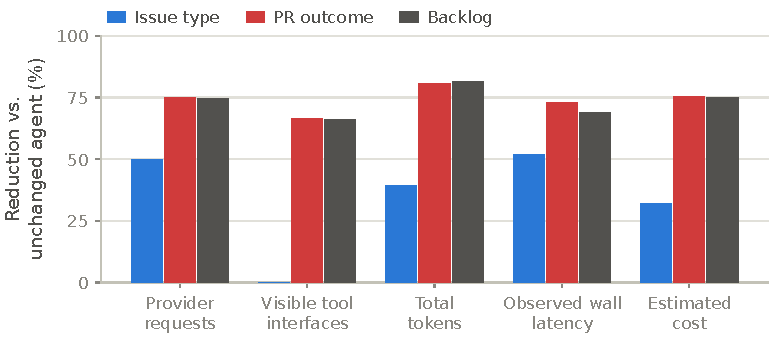
\includegraphics[width=0.8\linewidth]{figures/family_reductions.pdf}
  \caption{Per-family resource reductions behind \cref{tab:primary}, plotted
  because the spread is the result: admissible prefix depth --- not the
  optimizer --- sets the savings, and the two deeper families sit at the
  feasibility ceiling of \cref{eq:ceiling}.}
  \label{fig:family-reductions}
\end{figure}

\begin{figure}[t]
  \centering
  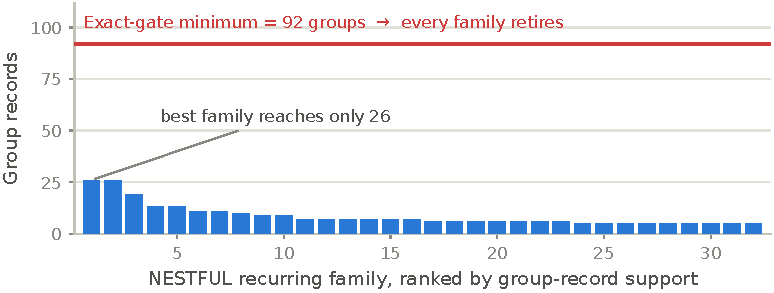
\includegraphics[width=0.9\linewidth]{figures/gate_support.pdf}
  \caption{NESTFUL family supports against the 92-group requirement implied by
  \cref{eq:cp} at $\alpha=0.05$, $\delta=0.1$, $|\Lambda|=11$. The largest family
  reaches 26 groups, so every family retires at calibration even though
  provenance, synthesis, and replay all succeeded.}
  \label{fig:gate-support}
\end{figure}

\Cref{fig:family-reductions} plots the per-family spread behind
\cref{tab:primary}: admissible prefix depth, not the optimizer, sets the
savings. The current empirical gate does not yet demonstrate a useful
risk--coverage frontier at the registered 5\% level. The strongest current runs are mostly
all-or-none support tests (\cref{fig:gate-support}), and the compiler-wide
candidate-search problem is not yet multiplicity-corrected. Likewise, exact task
contracts do not certify full semantic equivalence of the final answer,
especially once a downstream model continuation is involved. Two further
operational caveats belong in the record: the headline live artifact was
compiled without a sandbox available to the perturbation suite, so it records
\code{perturbations\_claimed: false} rather than a completed challenge, and
registry signature verification was configured off in the reported run. These
are not hidden defects in the repository; they are the reasons the paper avoids
stronger deployment claims.


\end{document}
